%************************************************
\chapter{Texture Features}\label{ch:texture}
%************************************************
\section{Introduction}
Texture is a household word outside image processing or related fields. However, in that context, it lacks a definition that allow us to measure and quantify it. Patter recognition provides us with a mathematical definition that allow us to use texture as a feature in our \ac{CAD} systems. 

Texture analysis is defined as any procedure by which we can quantify and classify the spatial variation of intensity throughout an image. In neuroimaging, texture has been widely used in segmentation (tissue classification) of \ac{MRI} images \cite{Saeed2002,Alejo2003,Wang2009}, although there exist a number of works using it for feature extraction in \ac{CAD}-like systems, like the works in \cite{kovalev2001three,sikio2015mr}, or our work on \ac{PKS} feature extraction \cite{Martinez-Murcia2013266,martinez2014parametrization}. 

Texture features can be classified in first, second and higher order analysis, depending on the number of variables used. First order statistics \cite{Martinez-Murcia2016b} are the most basic form of texture analysis, computing values such as average, variance or histogram of voxel intensity values \cite{Srinivasan2008}. 

The most popular form, with a very developed theoretical background, is second-order statistical texture analysis. This particular form is based on the probability of finding a pair of similar intensities at a certain distance and orientation of a certain image. From these probabilities, many measures can be derived, being the most popular the Haralick texture analysis \cite{Haralick73}. 

In this work we have used Haralick texture analysis to extract features from DaTSCAN images and perform an automatic diagnosis of \ac{PD}, as in \cite{Martinez-Murcia2013266,martinez2014parametrization}. First we will provide an introduction to the sub-volume selection procedure at Section~\ref{sec:volume}, and to the Haralick texture features at Section~\ref{sec:haralick}. Later, in Section~\ref{sec:ch5results} we define the experiments and show their results. Finally, at Section~\ref{sec:ch5discuss} we discuss the implications of this systems and the evaluation results of our texture-based \ac{CAD} system.

\section{Volume selection}\label{sec:volume}
Even the registered DaTSCAN images contain many voxels that are outside the brain. Therefore, to obtain a more robust estimation of the texture, it would be desirable to perform the computation of the features on subvolumes of those images (or subimages) that contain only voxels inside the brain. Many strategies can be performed for this, for example, force the computation of the \ac{GLCM} to ignore background voxels. 

In this work, we opted for extracting a subvolume which contains only voxels higher than a certain intensity threshold $I_{th}$, which should be specified. To do so, we obtain the maximum and minimum coordinates for which $\mathbf{I}$ is higher than the threshold: 
\begin{align}
	p_{x,min} & = \argmin_x \left( \mathbf{I} > I_{th} \right)\\
	p_{x,max} & = \argmax_x \left( \mathbf{I} > I_{th} \right)
\end{align}

And we do the same for the $y$ and $z$ axis of the array. Once this is computed, we can select the volume by: 

\begin{equation}
	\mathbf{I}_{sub} = \mathbf{I}[p_{x,min}:p_{x,max}, p_{y,min}:p_{y,max}, p_{z,min}:p_{z,max}]
\end{equation}

The resulting subvolume $\mathbf{I}_{sub}$ is the minimum box-shaped volume containing all the values for which $\mathbf{I}>I_{th}$, which allow us to select a $I_{th}$ so that only the regions of interest are contained within. 

Different subimages and sizes are obtained when applying different $I_{th}$ In Figure~\ref{fig:comparisonIth} we depict a comparison between the resulting images for $I_{th} = [0.25, 0.30, 0.35]$. 

\begin{figure}
	\centering
	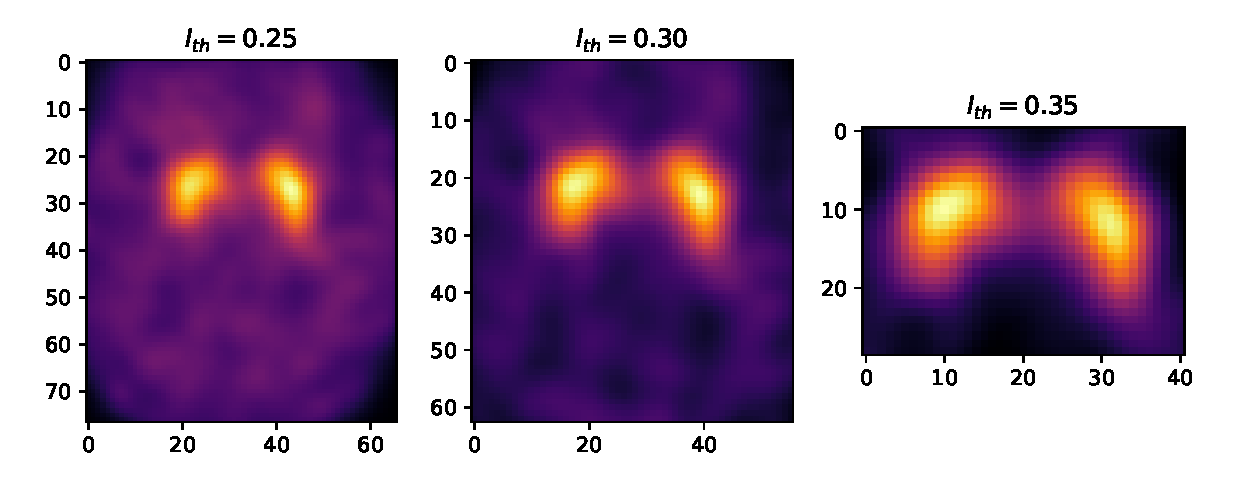
\includegraphics[width=0.90\columnwidth]{Graphics/ch5/comparisonIth.eps}
	\caption[Comparison of the different $I_{th}$ values.]{Comparison of the different $I_{th}$ values for a random subject extracted from the PPMI database.}
	\label{fig:comparisonIth}
\end{figure}



\section{Haralick Texture Features}\label{sec:haralick}
\subsection{Gray Level Co-occurrence Matrix}
%Que son las matriz de coocurrencia y las texture features
The Haralick texture analysis is based on the computation of a \acf{GLCM}, which is a form of evaluating second-order texture statistics. This matrix is a summary of the probabilities of finding a pair of similar grey levels at a certain distance and in a certain direction. 

The combination of the unitary vector dimension and the distance defines the offset $\Delta=(d_x,d_y,d_z)$, whose norm is the distance $d$ and is defined in a given spatial direction. In this work, we use a three-dimensional approach to the computation of the \ac{GLCM}, based on \cite{Philips2008}, that uses thirteen spatial directions to generalize the standard 2D \ac{GLCM} to 3D. These offset define different angles and are used to get some degree of rotational invariance \cite{Philips2008}. 

Medical images have different number precision, which can vary from regular 8bit integers (256 values) to the type float64 ($1.844\times10^{19}$ possible values). Using all these values, even in the smallest case, would lead to $256\times 256$ matrices, which would be both non representative of the real texture and computationally expensive. Therefore, prior to the \ac{GLCM} computation, we posterize the image, that is, the image is quantified to use only 16 grey levels. This leads to more tractable \ac{GLCM} without losing their representativeness. 

Once images have been posterized, for two different grey levels $i$ and $j$, the value of the co-occurrence matrix $\mathbf{C}$ over a $n \times m \times k$ three-dimensional image $\mathbf{I}$ is defined as: 
\begin{equation}\label{eq:cooc3D}
\mathbf{C}_{\Delta}(i,j)=\sum_{\mathbf{p}=(1,1,1)}^{(n,m,k)}\begin{cases} 1, & \mbox{if }\mathbf{I}(\mathbf{p})=i\mbox{ and }\mathbf{I}(\mathbf{p}+\Delta)=j \\ 0, & \mbox{otherwise}\end{cases}
\end{equation}
where $\Delta$ is the three dimensional offset that we defined previously, and $\mathbf{p}$ is the position of a given voxel inside the image. 

We will compute one $16\times16$ \ac{GLCM} for each of the combinations of direction and distances. This matrix $\mathbf{C}_{\Delta}$ is later modified to create the probability matrix $\mathbf{P}$ as: 
\begin{equation}
\mathbf{P}(i,j) = \frac{\mathbf{C}_{\Delta}(i,j)}{\sum_{i,j}\mathbf{C}_{\Delta}(i,j)}
\end{equation}
from which the texture features will be derived

\subsection{Haralick Texture Features}
%Parámetros de haralick. 
In \cite{Haralick73,Haralick1992a}, twelve texture features are derived from the probability matrix. These features are noted as:
\begin{align}
\text{Energy} & = \sum\limits_i\sum\limits_j \mathbf{P}(i,j)^2\\ 
\text{Entropy} & = \sum\limits_i\sum\limits_j \mathbf{P}(i,j) \log \mathbf{P}(i,j)\\
\text{Correlation} & = \frac{\sum_i\sum_j ij\mathbf{P}(i,j) - \mu_x\mu_y}{\sigma_x\sigma_y}\\
\text{Contrast} & = \sum\limits_{n=0}^{N_g-1} n^2 \left\lbrace\sum\limits_{|i-j|=n}\mathbf{P}(i,j)\right\rbrace  \\
\text{Variance} & \sum\limits_i\sum\limits_j (i-\mu_i)^2 \mathbf{P}(i,j)+ (j-\mu_j)^2\mathbf{P}(i,j)\\
\text{Sum Mean} & = \frac{1}{2} \sum\limits_i\sum\limits_j(i\mathbf{P}(i,j)+j\mathbf{P}(i,j))\\
\text{Inertia} & \sum\limits_i\sum\limits_j (i-j)^2\mathbf{P}(i,j)\\
\text{Cluster Shade} & \sum\limits_i\sum\limits_j (i+j-\mu_x-\mu_y)^3 \mathbf{P}(i,j)\\
\text{Cluster Tendency} & \sum\limits_i\sum\limits_j \{ i+j-\mu_x-\mu_y\}^4 \mathbf{P}(i,j)\\
\text{Homogeneity} & = \sum\limits_i\sum\limits_j \frac{\mathbf{P}(i,j)}{1+|i-j|}\\
\text{Max Probability} & = \max_{i,j} \mathbf{P}(i,j)\\
\text{Inverse Variance} & = \sum\limits_i\sum\limits_j {\mathbf{P}(i,j) \over (i-j)^2}
\end{align}
where $\mu_i$, $\mu_j$, $\sigma_i$ and $\sigma_j$ are the column and row-wise mean and variance respectively. These feature measure things such as the randomness of the grey-level distribution (entropy), the number of repeated pairs (energy), the local contrast or homogeneity of the image, variance, the tendency to form clusters (cluster shade and tendency), among others. 

For this work we have used a distance $d$ ranging from 1 to 10, at each of the $13$ spatial directions. Therefore, we have computed $13\times10=130$ \acp{GLCM} per image, from which $12$ texture features are computed. Our final feature vector will therefore have $1560$ features in total. 

To further reduce the dimensionality of the feature vector, we have performed feature selection using the $t$-test, \ac{MWW} $U$-test and the relative entropy (\ac{KL} divergence) criteria (see Section~\ref{sec:featureSelection}). 
% DONE

\section{Results}\label{sec:ch5results}
\subsection{Experiment 1}
In experiment 1, the influence and effect of using each of the twelve Haralick texture features on the results is tested, as in \cite{martinez2013texture}. GLC matrices are computed at a distance $d$ ranging from 1 to 10 voxels from the central one. As discussed later in this Section, the optimum sub-volume will have a smaller size than $40\times40\times50$, and so, the maximum value of $d=10$ correspond to at least $20\%$ of the brain sub-volume selected at that point; lower frequency textural changes can be neglected for diagnosis. Furthermore, as the voxel size of all databases is approximately 2x2x2mm, the maximum textural changes are computed within a 20x20x20mm area. This is approximately half the size of the striatum, which is enough to correctly extract the textural features of the area. 

The computed GLC matrices are used to extract the Haralick Texture Features in two different ways: a ''single approach'', which only considers one type of feature using only the matrices at a distance $d$ from the central voxel -and using all the spatial directions- and a ''cumulative approach'' which considers one type of feature too, but this time using all matrices in distances ranging from 1 to $d$. 

As commented before, we will use a normalization to the maximum strategy to normalize all the images in our three databases. After this, the 3D-GLC matrices will be computed over the selected subvolumes, given an intensity threshold $I_{th}$ (see Sec. \ref{sec:volume}). The optimum value of $I_{th}$ should be high enough to avoid introducing background voxels in the subvolume selected, yet adequately low to select the biggest subvolume containing only brain voxels. This should lead to the best performance, since the 3D GLC matrices (and the Haralick Texture Features) would have enough information, and would not include non-brain textural patterns. 

To better illustrate the influence of the subvolume selection process, Figure \ref{fig:featuresIth} depicts the average accuracy values for the two aforementioned approaches: Single (only the textural features computed at a distance $d$) and Cumulative (all textural features computed in the 1 to $d$ distance range). In both cases, 10 values of $d$, 13 directions and 12 features have been averaged to obtain the accuracy for each value of the intensity threshold $I_{th}$. 

\begin{figure*}% single and cumulative approach. 
	\centering
	\subfloat[Single approach]{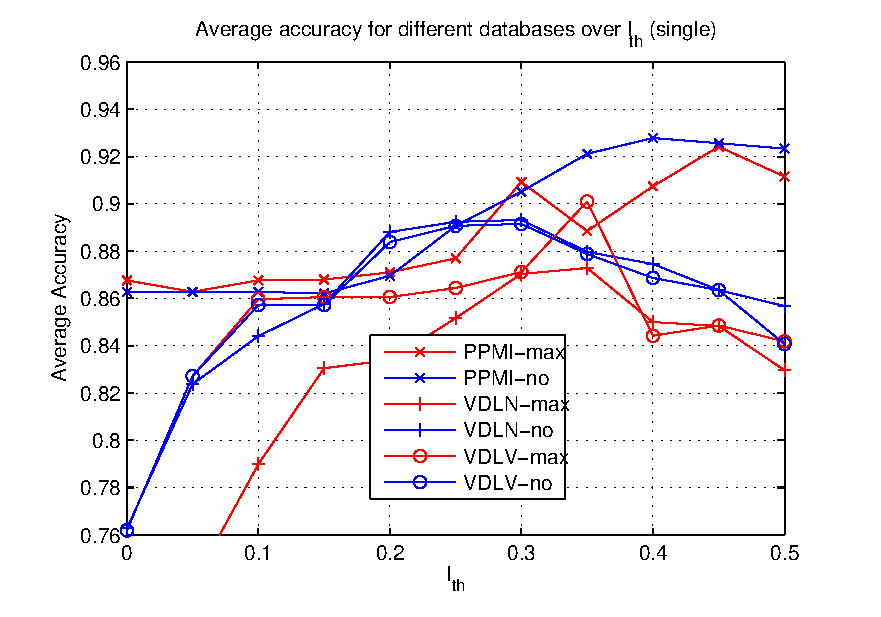
\includegraphics[width=0.45\textwidth]{Graphics/ch5/featuresIthdis.eps}\label{fig:acc_dist}}
	\subfloat[Cumulative approach]{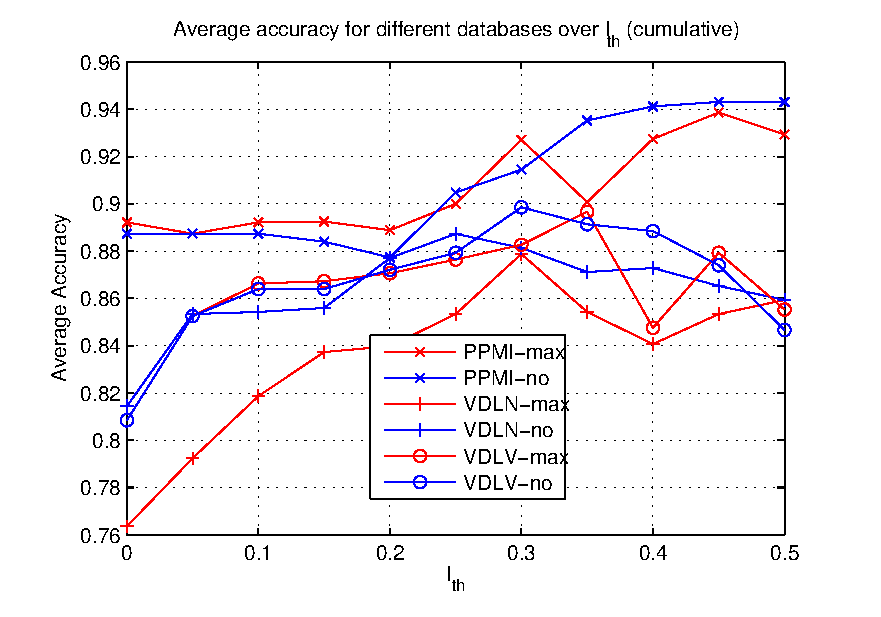
\includegraphics[width=0.45\textwidth]{Graphics/ch5/featuresIthcum.eps}\label{fig:acc_cum}}
	\caption{Average accuracy values obtained for \protect\subref{fig:acc_dist} the single approach and \protect\subref{fig:acc_cum} the cumulative approach.}
	\label{fig:featuresIth}
\end{figure*}

The effect of removing the background is clearly shown in these pictures, obtaining best results when using a $I_{th}>0.30\times I_{max}$ and then increasing the accuracy. Furthermore, the effect of the normalization is also clear in these two images. It is possible to notice that, when using no-normalized databases (those noted with a ``-no'' sufix) there are wide ranges of $I_{th}$ values in which similar performance values are obtained, while when using the normalized images, there are obvious peaks of accuracy around some values (usually, 0.30 or 0.35). Having applied no normalization to the images, the average image $I_{mean}$, from which the subvolume coordinates are extracted, is highly affected by the difference of intensities of different anatomical areas. Therefore, the subvolume computed will not be optimum, and for every value of $I_{th}$ there will be an set of samples in which the texture features will be correctly computed, and another set in which those will be poorly extracted. 

The behaviour of each of the Haralick texture features can also be analysed using a box plot (see Section \ref{sec:validation}), to show both numerical accuracy values and the properties (robustness, parameter independence) of using each one. Figure \ref{fig:features_acc_distances} depicts all $130$ accuracy results of the ''single approach'' for each feature extracted from a subimage that uses $I_{th}=0.30\times I_{max}$ at each distance $d$ (ranging from 1 to 10) in each of the 13 spatial directions. In this case, we can observe that best performance is obtained with the Cluster Tendency in all databases. Good values are also achieved using Homogeneity, Contrast and Correlation. This behaviour is consistent along all three databases, which allow us to propose Cluster Tendency as the best feature to characterize PD patterns. 

\begin{figure*}% Son los del experimento distances
	\centering
	\subfloat[PPMI database]{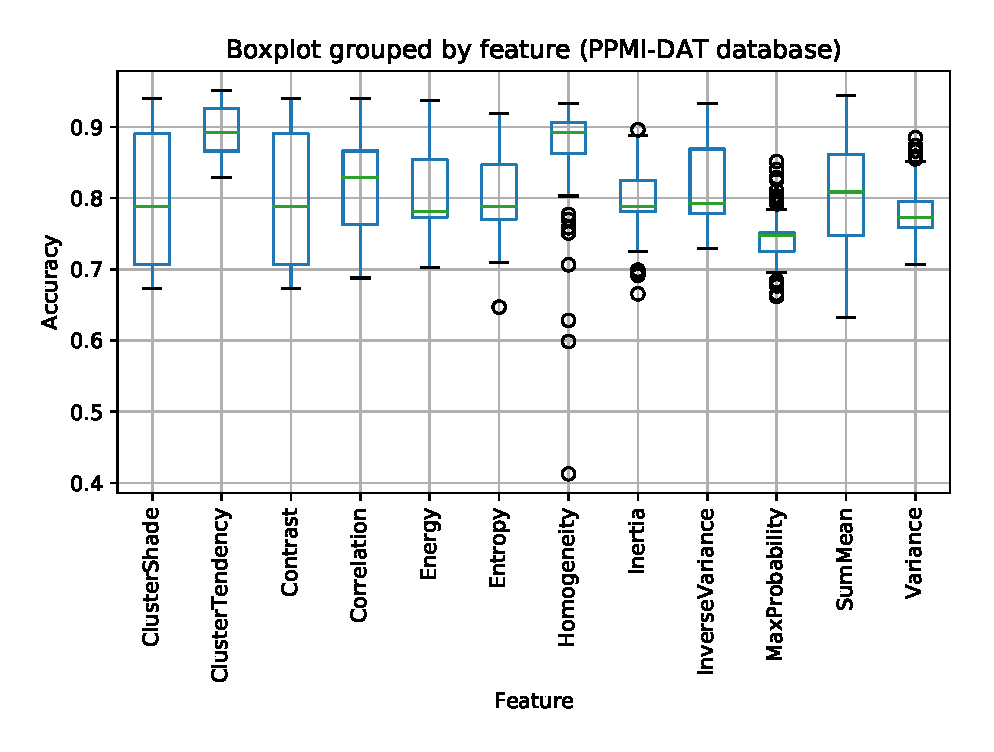
\includegraphics[height=0.25\textheight]{Graphics/ch5/features_accPPMI.eps}\label{fig:acc_distances_ppmi}}
	\subfloat[VDLN database]{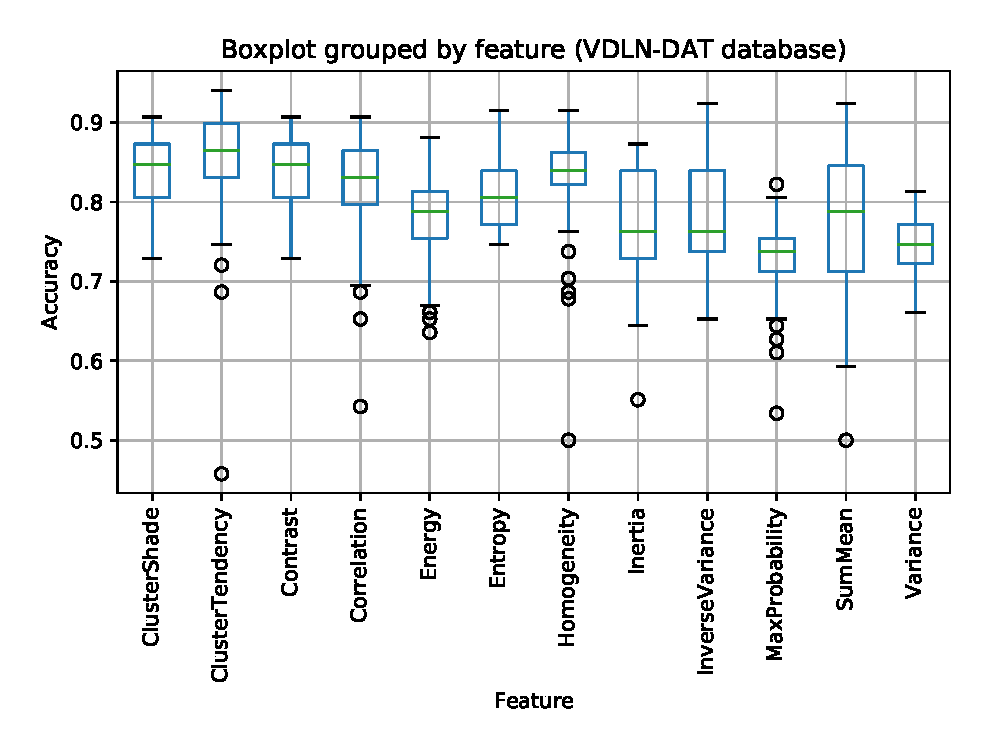
\includegraphics[height=0.25\textheight]{Graphics/ch5/features_accVDLN.eps}\label{fig:acc_distances_vdln}}
	\subfloat[VDLV database]{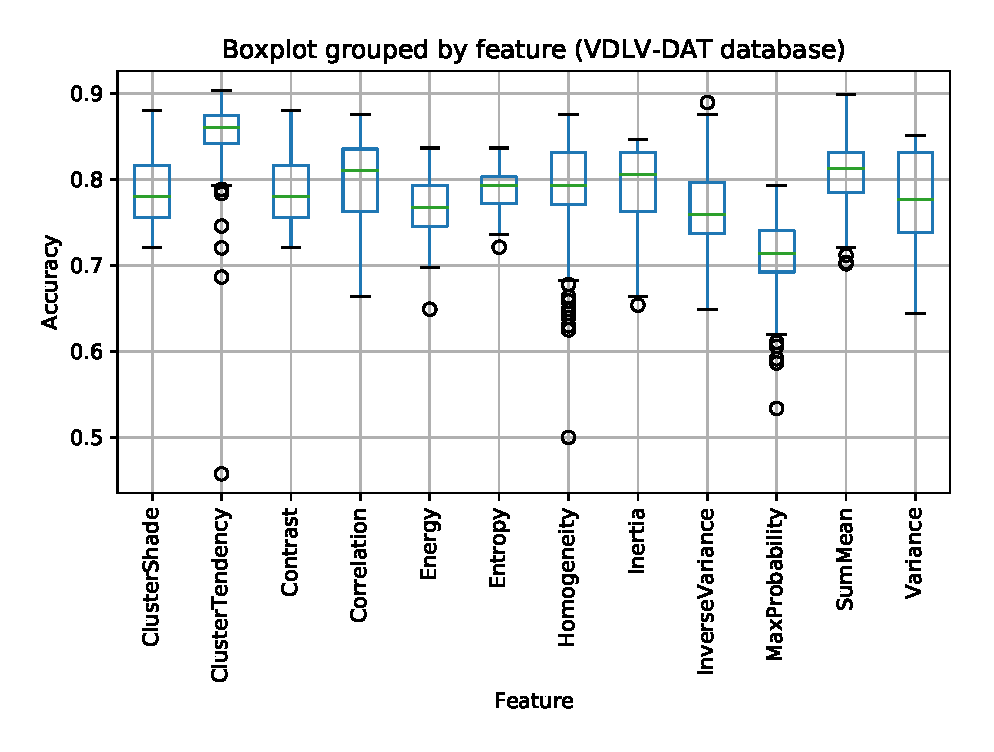
\includegraphics[height=0.25\textheight]{Graphics/ch5/features_accVDLV.eps}\label{fig:acc_distances_vdlv}}
	\caption{Box plot of all 130 accuracy values computed for each feature, using the ''single approach'', at 10 distances $d$ (ranging from 1 to 10) and 13 spatial directions, for \protect\subref{fig:acc_distances_ppmi} PPMI database, \protect\subref{fig:acc_distances_vdlv} VDLV database and \protect\subref{fig:acc_distances_vdln} VDLN database. The red marks represent the outliers.}
	\label{fig:features_acc_distances}
\end{figure*}

%The following step consists on evaluating the behaviour of this experiment when varying the distance $d$ at which the 3D GLC matrix is computed. 
%SOME MORE COMMENTS ON THIS. 
Finally, to characterize the ability of this single-feature approach, we show its performance at the defined operation point (Using an $I_{th}>0.30\times I_{max}$ and a value of $4<d<8$) in Table \ref{tab:exp1Acc}.

\begin{table*}[htp]
	\centering
	\begin{tabular}{llcccccccc}
		Database - approach & $I_{th}$	& $d$	& Feature	& Acc	& Sens	& Spec	& PL	& NL \\
		\hline\hline
		PPMI - cumulates	& 30	& 8	& Cluster Tendency	& 0.952	& 0.973	& 0.937	& 15.37	& 0.029 	 \\ % (5,1)
		PPMI - distances	& 30	& 6	& Cluster Tendency	& 0.952	& 0.964	& 0.943	& 16.92	& 0.038 	 \\ % (4,1)
		\hline
		VDLN - cumulates	& 30	& 6	& Cluster Tendency	& 0.906 & 0.911	& 0.904	& 9.50	& 0.098 	 \\ % (6,1)
		VDLN - distances	& 30	& 6	& Cluster Tendency	& 0.907	& 0.911	& 0.904	& 9.50	& 0.098 	 \\ % (7,1)
		\hline
		VDLV - cumulates	& 35	& 7	& Cluster Tendency	& 0.899 & 0.879	& 0.920	& 10.99	& 0.130 	 \\ % (6,1)
		VDLV - distances	& 35	& 6	& Cluster Tendency	&  0.923	& 0.907	& 0.940	& 15.12	& 0.098 	 \\ % (5,1)
		\hline\hline
	\end{tabular}
	\caption{Accuracy values obtained at the operation point, using Cluster Tendency as a feature. The $I_{th}$ used to compute the GLC matrix is also displayed. }
	\label{tab:exp1Acc}
\end{table*}

Obviously, the best approach is the cumulative one, given that it contains a bigger amount of information, and thus, describing in a more accurate way the different images. Note that for the cumulative approach, all values of Cluster Tendency computed between $d=1$ and $d$ are used, while for the single approach, only values of Cluster Tendency at $d$ are considered. However, the single approach also performs relatively well, proving the value of the Haralick texture features to characterize DaTSCAN images. 

Results are particularly good in every case when $I_{th} > 0.30\times I_{max}$, a phenomenon that was previously shown in PPMI database (see Fig. \ref{fig:featuresIth}), but that also extends here to all other databases. 


\subsection{Experiment 2}
For experiment 2, all features computed in the aforementioned experiments (the 13 direction vectors and 10 distances used to compute the 3D coocurrence matrix, and the 12 Haralick texture features extracted from these matrices) are used as an input to the classifier. But, in order to reduce dimensionality, we use the measures of discrimination ability proposed in Section \ref{sec:discrimination} to rank these features in a descending order of ability in distinguish PD patterns from normal controls, selecting the first $N$. 

Firstly, the impact of our volume selection threshold $I_{th}$ (see Sec. \ref{sec:volume}) on the quality of the resulting Haralick Features, and thus, the accuracy of the experiment, will be analysed. As commented before, best results should be obtained when taking into account the biggest volume of the brain containing only brain voxels, and thus, eliminating the background. Regarding all databases, we obtain Figure \ref{fig:averageAcc_IthNorm}, in which average values of accuracy for every value of $I_{th}$ are plotted. These average values are computed in a similar way to Fig. \ref{fig:featuresIth}, by averaging all $50$ accuracy values that correspond to each value of $I_{th}$. The accuracy values are obtained using each of the 5 proposed selection methods, and using each value of percentage of features selected (ranging from 1 to 100\%, by steps of 10\%, of the total amount of 1560 features). 

\begin{figure}[htp]
	\centering
	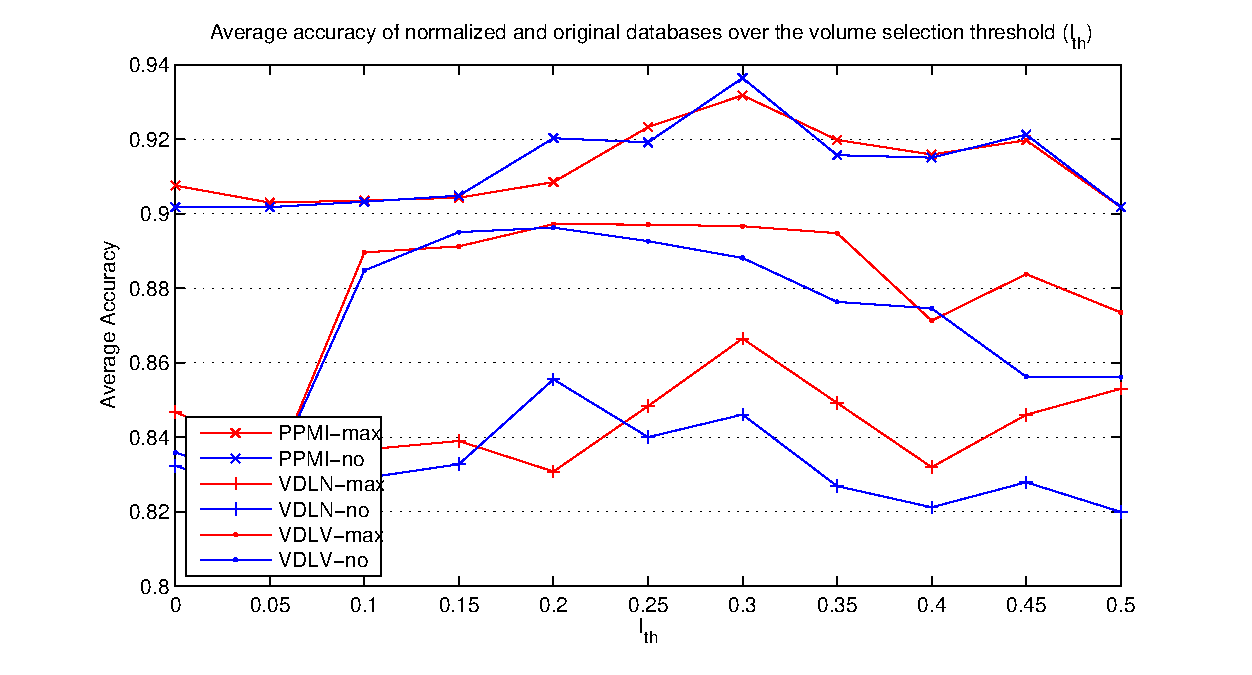
\includegraphics[width=0.90\columnwidth]{Graphics/ch5/accuracyOverIth.eps}
	\caption{Accuracy obtained by averaging all accuracy values using a given volume selection threshold $I_{th}$}
	\label{fig:averageAcc_IthNorm}
\end{figure}

For two out of three databases there is a clear maximum in accuracy for an $I_{th} = 0.30\times I_{max}$, while the remaining one obtain similar results along a wide range of $I_{th}$. Furthermore, best average values are obtained using the normalized database, although the PPMI case is slightly different, due to the attenuation correction preprocessing. In Fig. \ref{fig:cut_thr30} the resulting subimage of applying this threshold was shown, to provide a better understanding of how the textural features are better defined in this. As suggested before, all no-brain voxels are removed from this images, all the textural features correspond only to the internal brain textural changes, and thus, to the textural patterns of the disease, leading to a better performance. 

As results suggest, the use of our volume selection strategy with a intensity threshold between $0.25$ and $0.45$ is profitable in all cases. Also, the use of intensity normalized images, using the normalization to the maximum algorithm has also a good impact on the performance of the system. In this context, Fig. \ref{fig:experiment4} analyses the behavior of our system using each of the discrimination-based ranking methods. On these three figures, the values of the computed average accuracy (using the values for intensity thresholds of $0.10$ to $0.45$) are plotted over the percentage of selected features (previously ranked from the most to the least discriminant, following different criteria) using the three databases. 

\begin{figure*}
	\centering
	\subfloat[PPMI database]{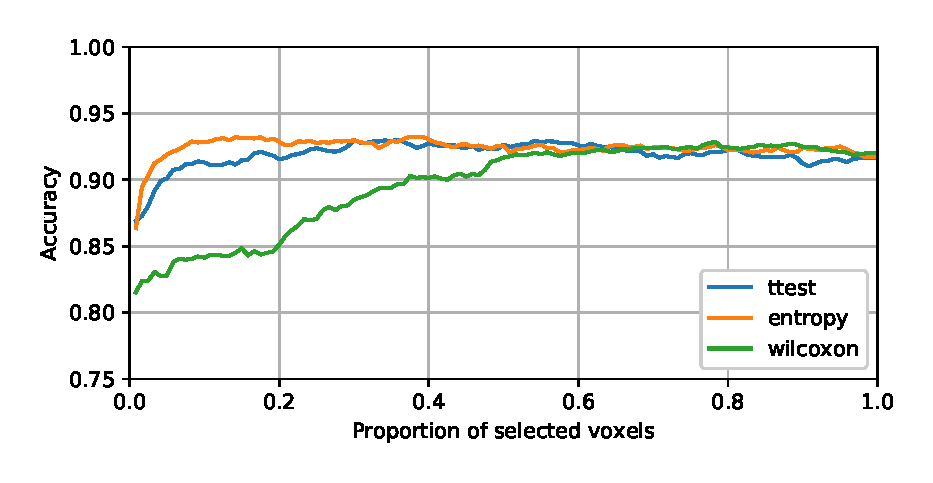
\includegraphics[width=0.45\textwidth]{Graphics/ch5/features_avAccPPMI.eps}\label{fig:experiment4-ppmi}}
	\subfloat[VDLN database]{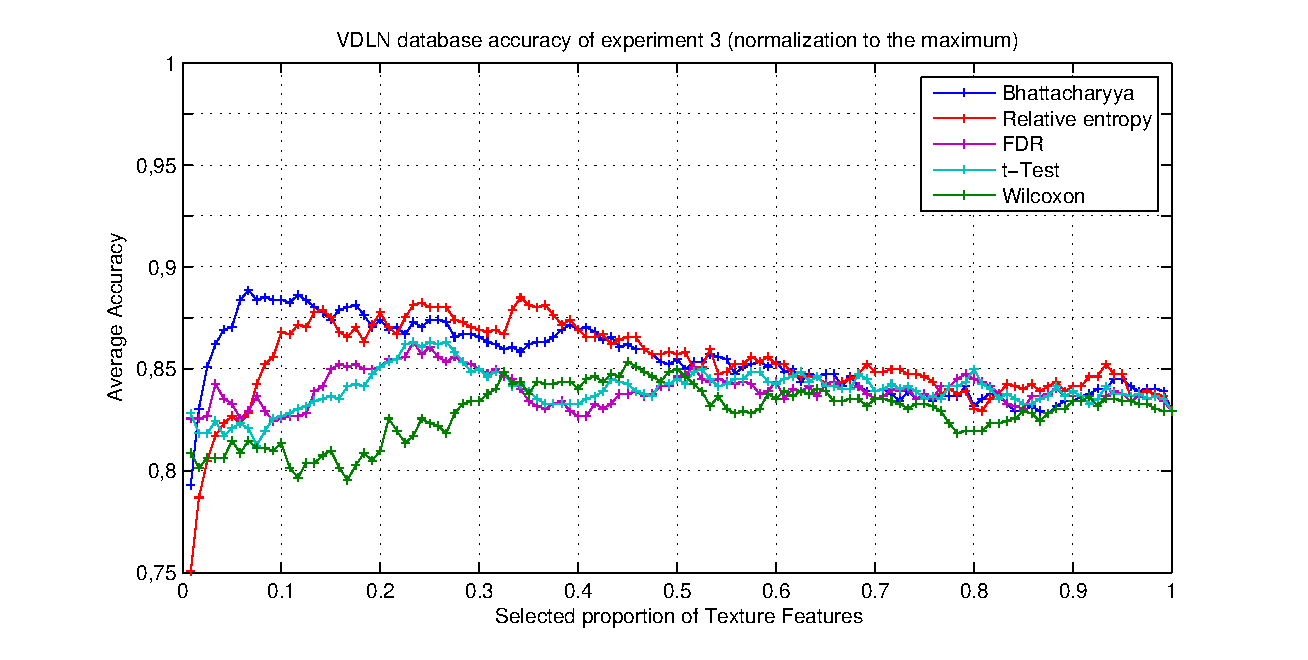
\includegraphics[width=0.45\textwidth]{Graphics/ch5/features_avAccVDLN.eps}\label{fig:experiment4-vdln}}
	\subfloat[VDLV database]{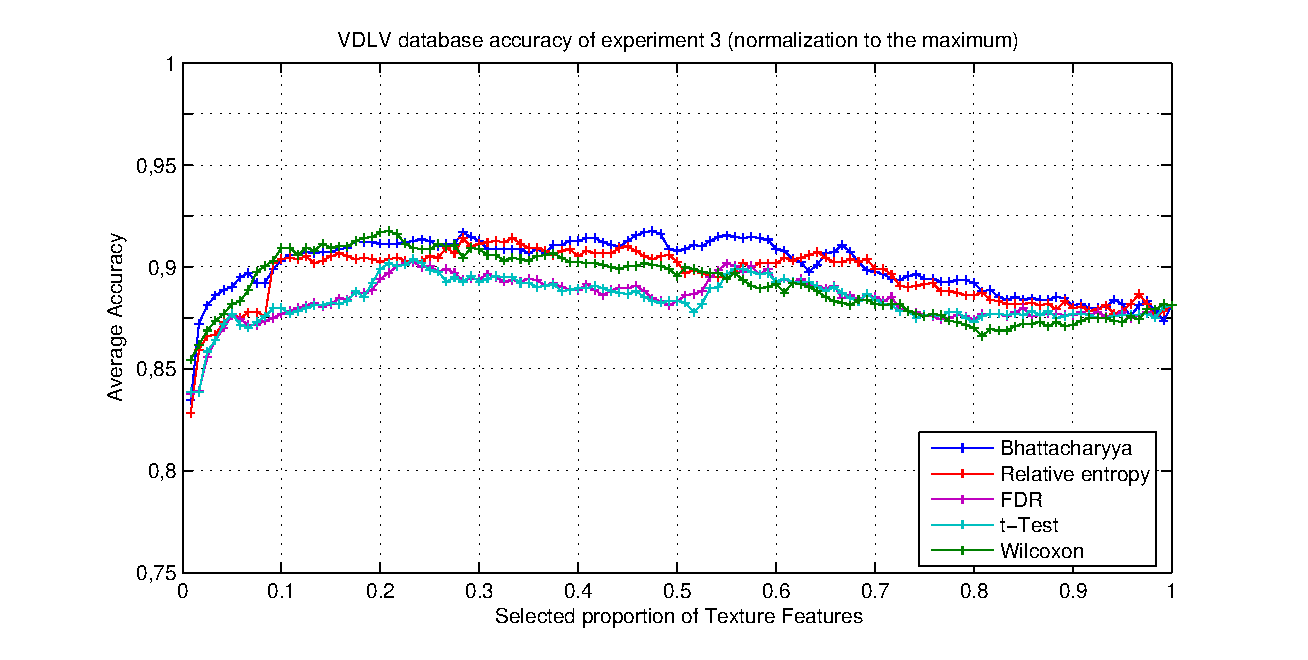
\includegraphics[width=0.45\textwidth]{Graphics/ch5/features_avAccVDLV.eps}\label{fig:experiment4-vdlv}}
	\caption{Average accuracy computed for each selection criteria, using all accuracy values for intensity thresholds of $0.10$ to $0.45$. These values are plotted over $N$, the number of features selected using some of the ranking criteria defined in Sec. \ref{sec:discrimination} (where $N$ ranges from 1\% and 100\% of the $1560$ total Haralick features calculated). These values correspond to the images of the \protect\subref{fig:experiment4-ppmi} PPMI database, \protect\subref{fig:experiment4-vdlv} VDLV database and \protect\subref{fig:experiment4-vdln} VDLN database (experiment 2).}
	\label{fig:experiment4}
\end{figure*}

Some conclusions about the amount of features that each of our discrimination-ranking methods need can be extracted from these average accuracy graphs. Methods that obtain their maximum accuracy using less than 50\% of the features can be considered of great help, as they perform a significant feature reduction. Therefore, methods like Mann-Whitney-Wilcoxon (MWW) can no longer be considered, as it needs more than 50\% of features to obtain good results. The opposite behaviour is given by Bhattacharyya Distance (BD) and Relative Entropy (RE), that obtain their maximum average accuracy using the first 10\% of features. Fisher's Discriminant Ratio (FDR) and $t$-Test need a higher amount, but less than 50\%. 

The aforementioned behaviour correspond to an average behaviour in accuracy. To take a deeper look at the different evaluation parameters and different selection criteria, peak results obtained with each selection criteria are shown on Table \ref{tab:exp3Res}. 

\begin{table*}[htp]
	\centering
	\begin{tabular}{llcccccc}
		Database 	 & Criterium	& Accuracy	& Sensitivity	& Specificity	& PL	& NL	& \% \\
		\hline \hline
		\multirow{5}{*}{\textbf{PPMI}}	& Bhattacharyya	& 0.967	& 0.973	& 0.962	& 25.62	& 0.028	& 49.1\\ % (59,1)
		& Relative Entropy	& 0.967	& 0.982	& 0.956	& 22.16	& 0.019 & 30.8\\ % (37,1)
		& FDR	& 0.974	& 0.991	& 0.962	& 26.10	& 0.009 & 34.2\\ % (41,1)
		& $t$-Test	& 0.974	& 0.991	& 0.962	& 26.10	& 0.009 & 35.8\\ % (43,1)
		& Wilcoxon	& 0.959	& 0.955	& 0.962	& 25.15	& 0.047 & 85.8\\ % (103,1)
		\hline
		\multirow{5}{*}{\textbf{VDLN}} &  Bhattacharyya	& 0.924	& 0.956	& 0.904	& 9.97	& 0.049 & 10.0\\ % (12,1
		& Relative Entropy	& 0.924	& 0.933	& 0.918	& 11.36	& 0.073 & 20.0\\ % (24,1)
		& FDR	& 0.941	& 0.933	& 0.945	& 17.03	& 0.071 & 16.7\\ % (20,1)
		& $t$-Test	& 0.932	& 0.933	& 0.932	& 13.63	& 0.072 & 22.5\\ % (27,1)
		& Wilcoxon	& 0.898	& 0.889	& 0.904	& 9.27	& 0.123 & 3.3\\ % (4,1)
		\hline
		\multirow{5}{*}{\textbf{VDLV}}	& Bhattacharyya	& 0.938	& 0.935	& 0.940	& 15.59	& 0.069 & 40.8\\ % (49,1)
		& Relative Entropy	& 0.933	& 0.935	& 0.930	& 13.36	& 0.070 & 45.8\\ % (55,1)
		& FDR	& 0.928	& 0.963	& 0.890	& 8.75	& 0.042 & 30.8 \\ % (37,1)
		& $t$-Test	& 0.933	& 0.935	& 0.930	& 13.36	& 0.070 & 34.2\\ % (41,1)
		& Wilcoxon	& 0.928	& 0.926	& 0.930	& 13.23	& 0.080 & 18.3\\ % (22,1)
		
		\hline\hline
	\end{tabular}
	\caption{Best results obtained in experiment 2, using three databases, in terms of its accuracy, sensitivity, specificity, Positive Likelihood and Negative Likelihood. The amount of features used to achieve these results is shown as a percentage of the total number of features (1560). Values obtained by leave-one-out.}
	\label{tab:exp3Res}
\end{table*}

This table confirms that the Mann-Whitney-Wilcoxon method can be no longer considered, as it needs more than a 50\% of the features to obtain poorer results than all others. Regarding the remaining methods, we observe that those that needed a lower amount of features (BD and RE) obtain here lower values of accuracy that those that needed a higher amount ($t$-Test and FDR). So, the choice of the best method is, in this case, a matter of trade-off between the computer performance (the number of features to estimate) and the accuracy needed. As in clinical practice, accuracy (and PL) is the parameter that needs to be maximized, we can conclude that FDR and $t$-Test are the best discrimination-ranking methods to use in this task, although all other methods reveal the ability of our system in the PD detection with an relevant performance (over 90\% of accuracy in most cases). 

For comparison purposes, we have established a baseline method proposed in Illan et al \cite{Illan2012}, where a Voxels-as-Features (VAF) approach with SVM linear, using different normalization strategies were tested. Two additional methods have been compared with our proposed system in order to check the performance versus state-of-the-art algorithms. These methods have been an asymmetrical Single Value Decomposition (SVD) \cite{Segovia2012} that appplied SVD on both sides of the brain (since PD often appears only in one hemisphere), and a Empirical Mode Decomposition (EMD)  \cite{Rojas2012} using different Independent Mode Functions (IMF), particularly the IMF-3. Table \ref{tab:comparison} compares all the aforementioned methods. 

\begin{table*}[ht]
	\centering
	\begin{tabular}{l | rrrrr}
		\hline\hline
		\textbf{System}		& \textbf{Acc} 	& \textbf{Sens}	& \textbf{Spec}	& \textbf{PL}	& \textbf{NL}\\ 
		\hline
		Homogeneity & 0.959 & 0.973 & 0.949 & 19.22 & 0.028\\
		Cluster Shade & 0.955 & 0.964 & 0.949 & 19.01 & 0.038\\
		Cluster Tendency & 0.955 & 0.973 & 0.943 & 17.10 & 0.029\\
		Correlation & 0.941 & 0.946 & 0.937 & 14.92 & 0.058\\
		Energy & 0.937 & 0.964 & 0.918 & 11.73 & 0.039\\
		\hline
		Entropy	& 0.967	& 0.982	& 0.956	& 22.16	& 0.019 \\ % (37,1)
		FDR	& 0.974	& 0.991	& 0.962	& 26.10	& 0.009 \\ % (41,1)
		$t$-Test	& 0.974	& 0.991	& 0.962	& 26.10	& 0.009 \\ % (43,1)
		\hline
		VAF & 0.840	& 0.807	& 0.862	& 5.88	& 0.224 \\
		VAF-IN & 0,913 & 0.890 & 0.932 & 13.08 & 0.118\\
		SVD & 0.940 & 0.962 & 0.918 & 11.73 & 0.041\\
		EMD-IMF3 & 0.950 & 0.951 & 0.948 & 18.28 & 0.051\\
		\hline\hline
	\end{tabular}
	\vspace{10pt}
	\caption{Comparison of our proposed system (using different texture features) and some other methods in the bibliography: VAF system using the intensity-normalized images,  a combination of intensity normalization strategies and classifiers (VAF-IN) \cite{Illan2012}, a SVD-based approach \cite{Segovia2012} and EMD using the third independent mode function (IMF3) \cite{Rojas2012}.}
	\label{tab:comparison}
\end{table*}

In Table \ref{tab:comparison}, performance values at the operation point are shown for Experiment 1 (using five texture features: Homogeneity, Cluster shade, Cluster tendency, Correlation and energy) and for Experiment 2 (using Relative Entropy, FDR or Student's $t$-Test). These values are compared with the VAF, SVD and EMD approaches previously cited. We can observe that the performance values obtained with Experiment 1 are very similar to other state-of-the-art methods, like the proposed in \cite{Segovia2012,Rojas2012}, whereas the methodology used in Experiment 2 outperform all previously used methods. Particularly, as we previously mentioned, the use of either FDR or $t$-Test to select the most discriminant features gives us results over a PL of $26$ and sensitivity over $99\%$, which proves the ability of some Haralick Textures, and the combination of them, in characterizing the different Parkinson's Disease patterns, and the robustness of the proposed methods. 
\section{Discussion}\label{sec:ch5discuss}